\documentclass[aspectratio=169]{beamer}
\usetheme{Madrid}
\usecolortheme{default}

\usepackage{graphicx}
\usepackage{amsmath}
\usepackage{booktabs}
\usepackage{tikz}
\usetikzlibrary{shapes,arrows,positioning}

% Custom colors
\definecolor{uniblue}{RGB}{0,51,102}
\definecolor{unigreen}{RGB}{0,128,0}
\setbeamercolor{structure}{fg=uniblue}

% Override background for specific slides
\newcommand{\whitebg}{%
    \setbeamercolor{background canvas}{bg=white}%
    \setbeamercolor{normal text}{fg=black}%
    \usebeamercolor[fg]{normal text}%
}

% Title page info
\title[Ethical AI Storyteller]{Ethical AI Storyteller}
\subtitle{Integrating Safety, Bias Mitigation, and Explainability in Neural Story Generation}
\author[Salihu, Mustafa, Hoxha]{Eron Salihu \and Miran Mustafa \and Urim Hoxha}
\institute[UP]{
    Faculty of Electrical and Computer Engineering\\
    University of Prishtina ``Hasan Prishtina''\\
    \vspace{0.3cm}
    Natural Language Processing Course\\
    Instructor: Dr. Sc. Mërgim H. HOTI
}
\date{December 2025}

\begin{document}

% Title slide
\begin{frame}
    \titlepage
\end{frame}

% Outline
\begin{frame}{Outline}
    \tableofcontents
\end{frame}

% Section 1: Introduction
\section{Introduction}

\begin{frame}{Motivation}
    \begin{block}{The Challenge}
        Large language models can generate fluent narratives but face critical challenges:
        \begin{itemize}
            \item \textbf{Safety:} Risk of producing toxic or harmful content
            \item \textbf{Bias:} Amplification of societal stereotypes
            \item \textbf{Transparency:} Black-box decision making
        \end{itemize}
    \end{block}
    
    \vspace{0.5cm}
    
    \begin{block}{Our Solution}
        An integrated system that combines story generation with:
        \begin{itemize}
            \item Multi-layer ethical filtering
            \item Pattern-based bias detection
            \item Explainability mechanisms
        \end{itemize}
    \end{block}
\end{frame}

\begin{frame}{Project Contributions}
    \begin{enumerate}
        \item \textbf{Modular Storyteller}
        \begin{itemize}
            \item GPT-2 generation with layered ethical filtering
            \item Real-time bias detection
        \end{itemize}
        
        \vspace{0.3cm}
        
        \item \textbf{Built-in Explainability}
        \begin{itemize}
            \item Attention heatmaps
            \item Token importance analysis
            \item Next-token diagnostics
        \end{itemize}
        
        \vspace{0.3cm}
        
        \item \textbf{Reproducible Pipeline}
        \begin{itemize}
            \item Fine-tuning support
            \item Offline evaluation
            \item 50-story local dataset
        \end{itemize}
        
        \vspace{0.3cm}
        
        \item \textbf{Interactive Interface}
        \begin{itemize}
            \item Real-time Gradio web application
            \item Safety ratings and bias alerts
        \end{itemize}
    \end{enumerate}
\end{frame}

% Section 2: System Architecture
\section{System Architecture}

\begin{frame}{System Overview}
    \begin{center}
        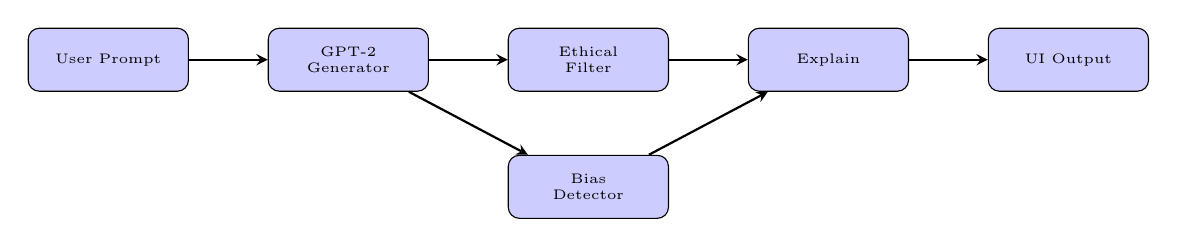
\begin{tikzpicture}[
            node distance=1.0cm,
            block/.style={rectangle, draw, fill=blue!20, text width=1.8cm, text centered, rounded corners, minimum height=0.8cm, font=\tiny},
            arrow/.style={->, >=stealth, thick}
        ]
            \node[block] (prompt) {User Prompt};
            \node[block, right=of prompt] (generator) {GPT-2\\Generator};
            \node[block, right=of generator] (filter) {Ethical\\Filter};
            \node[block, below=0.8cm of filter] (bias) {Bias\\Detector};
            \node[block, right=of filter] (explain) {Explain};
            \node[block, right=of explain] (output) {UI Output};
            
            \draw[arrow] (prompt) -- (generator);
            \draw[arrow] (generator) -- (filter);
            \draw[arrow] (filter) -- (explain);
            \draw[arrow] (explain) -- (output);
            \draw[arrow] (generator) -- (bias);
            \draw[arrow] (bias) -- (explain);
        \end{tikzpicture}
    \end{center}
    

\end{frame}

\begin{frame}{Core Modules}
    \begin{columns}
        \begin{column}{0.5\textwidth}
            \begin{block}{Generation \& Processing}
                \begin{itemize}
                    \item \texttt{story\_generator.py}
                    \begin{itemize}
                        \small
                        \item GPT-2 models
                        \item 8 genre support
                        \item Nucleus sampling
                    \end{itemize}
                    
                    \item \texttt{dataset.py}
                    \begin{itemize}
                        \small
                        \item HuggingFace datasets
                        \item Local JSON stories
                    \end{itemize}
                    
                    \item \texttt{finetune.py}
                    \begin{itemize}
                        \small
                        \item Training pipeline
                        \item Checkpointing
                    \end{itemize}
                \end{itemize}
            \end{block}
        \end{column}
        
        \begin{column}{0.5\textwidth}
            \begin{block}{Ethics \& Transparency}
                \begin{itemize}
                    \item \texttt{ethical\_filter.py}
                    \begin{itemize}
                        \small
                        \item Detoxify integration
                        \item Pattern matching
                        \item 5-level rating
                    \end{itemize}
                    
                    \item \texttt{explainability.py}
                    \begin{itemize}
                        \small
                        \item Attention visualization
                        \item Token importance
                    \end{itemize}
                    
                    \item \texttt{storyteller.py}
                    \begin{itemize}
                        \small
                        \item Main orchestrator
                        \item Retry logic
                    \end{itemize}
                \end{itemize}
            \end{block}
        \end{column}
    \end{columns}
\end{frame}

% Section 3: Datasets
\section{Datasets}

\begin{frame}{Datasets Overview}
    \begin{table}
        \centering
        \small
        \begin{tabular}{lccc}
            \toprule
            \textbf{Dataset} & \textbf{Source} & \textbf{Samples} & \textbf{Size} \\
            \midrule
            WritingPrompts & HuggingFace & 500--1000 & \textasciitilde50MB \\
            TinyStories & HuggingFace & 500--1000 & \textasciitilde30MB \\
            FairyTales & HuggingFace & 200--500 & \textasciitilde15MB \\
            \textbf{Local Dataset} & Custom & \textbf{50} & \textbf{45KB} \\
            \bottomrule
        \end{tabular}
    \end{table}
    
    \vspace{0.5cm}
    
    \begin{block}{Local Dataset Characteristics}
        \begin{itemize}
            \item \textbf{Purpose:} Offline reproducibility for grading
            \item \textbf{Genres:} Fantasy (20\%), Sci-Fi (18\%), Mystery (16\%), Adventure (16\%), Romance (16\%), Horror (14\%)
            \item \textbf{Format:} JSON with id, genre, prompt, story
        \end{itemize}
    \end{block}
\end{frame}

% Section 4: Methodology
\section{Methodology}

\begin{frame}{Story Generation}
    \begin{block}{Model Variants}
        \begin{itemize}
            \item GPT-2 (124M) -- default for efficiency
            \item GPT-2 Medium (355M)
            \item GPT-2 Large (774M)
            \item DistilGPT-2 (82M) -- fastest inference
        \end{itemize}
    \end{block}
    
    \vspace{0.3cm}
    
    \begin{block}{Generation Parameters}
        \begin{columns}
            \begin{column}{0.5\textwidth}
                \begin{itemize}
                    \item Nucleus sampling ($p=0.95$)
                    \item Top-$k$ = 50
                    \item Temperature = 0.8--1.0
                \end{itemize}
            \end{column}
            \begin{column}{0.5\textwidth}
                \begin{itemize}
                    \item Repetition penalty = 1.2
                    \item 3-gram blocking
                    \item Max length = 200 tokens
                \end{itemize}
            \end{column}
        \end{columns}
    \end{block}
\end{frame}

\begin{frame}{Multi-Layer Ethical Filtering}
    \whitebg
    {\small
    \textbf{Layer 1: ML-Based Toxicity Detection}
    
    \textbf{Detoxify} with thresholds: toxicity 0.5, severe 0.3
    \begin{itemize}
        \item Detects: hate speech, threats, identity attacks, obscenity
    \end{itemize}
    
    \vspace{0.3cm}
    
    \textbf{Layer 2: Pattern-Based Blocking}
    
    Regex patterns for explicit harmful content
    \begin{itemize}
        \item Violence, discrimination, self-harm keywords
    \end{itemize}
    
    \vspace{0.3cm}
    
    \textbf{Layer 3: Prosocial Encouragement}
    
    Detects positive elements: friendship, hope, courage, kindness
    }
\end{frame}

\begin{frame}{Content Rating System}
    \whitebg
    {\small
    \[
    \text{rating}(y) = f_{\text{safety}}(y;\tau) \in \left\{
    \begin{array}{l}
    \text{Safe}\\
    \text{Mild}\\
    \text{Moderate}\\
    \text{Restricted}\\
    \text{Blocked}
    \end{array}
    \right\}
    \]
    
    \vspace{0.2cm}
    
    \begin{itemize}
        \item \textbf{Blocked patterns} $\rightarrow$ BLOCKED
        \item \textbf{High toxicity} (>0.8) $\rightarrow$ BLOCKED
        \item \textbf{Moderate toxicity} (0.6--0.8) $\rightarrow$ RESTRICTED
        \item \textbf{Sensitive topics} $\rightarrow$ MODERATE/MILD
        \item \textbf{Positive content} (3+ cues) $\rightarrow$ SAFE
    \end{itemize}
    

    \begin{alertblock}{Retry Mechanism}
        Re-generates (max 3 attempts) with increased temperature if unacceptable.
    \end{alertblock}
    }
\end{frame}

\begin{frame}{Bias Detection}
    \whitebg
    {\footnotesize
    \textbf{Pattern-Based Approach}
    
    Identifies stereotypes in generated text:
    
    \begin{table}
        \centering
        \tiny
        \begin{tabular}{ll}
            \toprule
            \textbf{Category} & \textbf{Example Patterns} \\
            \midrule
            Gender roles & ``women should...'', ``men must...'' \\
            Profession & ``woman nurse'', ``man engineer'' \\
            Trait & ``emotional woman'', ``tough man'' \\
            \bottomrule
        \end{tabular}
    \end{table}
    
    \vspace{0.3cm}
    
    \textbf{Actionable Recommendations}
    
    When bias detected:
    \begin{itemize}
        \item Specific category identified
        \item Suggestions for balanced representations
        \item Warning in UI
    \end{itemize}
    }
\end{frame}

\begin{frame}{Explainability Methods}
    \whitebg
    {\footnotesize
    \textbf{1. Attention Visualization}
    
    Heatmaps showing token attention (selectable layer)
    
    \vspace{0.3cm}
    
    \textbf{2. Leave-One-Out Token Importance}
    
    Measures contribution via KL divergence:
    \[
    \text{importance}(t_i) = D_{KL}(P_{\text{baseline}} \| P_{\text{masked}})
    \]
    
    \vspace{0.3cm}
    
    \textbf{3. Next-Token Prediction}
    
    Top-k candidates with probability distribution
    }
\end{frame}

% Section 5: Implementation
\section{Implementation}

\begin{frame}{Web Interface (Gradio)}
    \whitebg
    {\small
    \textbf{Interactive Features}
    
    \textbf{Tab 1: Generate Story}
    \begin{itemize}
        \item Genre selection, parameter tuning, safety ratings
    \end{itemize}
    
    \textbf{Tab 2: Continue Story}
    \begin{itemize}
        \item Extend existing narratives with coherence
    \end{itemize}
    
    \textbf{Tab 3: Explain}
    \begin{itemize}
        \item Next-token predictions, attention heatmaps, token importance
    \end{itemize}
    
    \textbf{Tab 4: Safety Check}
    \begin{itemize}
        \item Analyze any text with detailed toxicity scores
    \end{itemize}
    }
\end{frame}

\begin{frame}{Offline Mode \& Reproducibility}
    \whitebg
    {\small
    \textbf{Designed for Coursework}
    \begin{itemize}
        \item \textbf{Offline operation:} Works without internet
        \item \textbf{Local dataset:} 50-story JSON bundle
        \item \textbf{Graceful fallback:} Regex-only if Detoxify unavailable
        \item \textbf{Model caching:} Pre-download for grading
    \end{itemize}
    
    \vspace{0.3cm}
    
    \textbf{Testing Strategy}
    \begin{itemize}
        \item \textbf{Unit tests:} Mocked modules (no large model loading)
        \item \textbf{Smoke tests:} Dataset loading, offline init
        \item \textbf{Benchmarks:} Optional execution
    \end{itemize}
    }
\end{frame}

% Section 6: Evaluation
\section{Evaluation}

\begin{frame}{Evaluation Metrics}
    \whitebg
    {\small
    \textbf{Perplexity (PPL)}
    
    Measures model confidence (lower is better):
    \[
    \text{PPL} = \exp\left(-\frac{1}{N}\sum_{i=1}^{N} \log P(\text{token}_i | \text{context})\right)
    \]
    
    \vspace{0.3cm}
    
    \textbf{Safe Content Ratio}
    
    Proportion passing safety filters:
    $\text{Safe Ratio} = \text{safe\_count} / \text{total\_count}$
    
    \vspace{0.3cm}
    
    \textbf{Bias Ratio}
    
    Proportion with detected stereotypes:
    $\text{Bias Ratio} = \text{biased\_count} / \text{total\_count}$
    }
\end{frame}

\begin{frame}{Results: Model Comparison}
    \begin{table}
        \centering
        \begin{tabular}{lccc}
            \toprule
            \textbf{Model} & \textbf{PPL} $\downarrow$ & \textbf{Safe} $\uparrow$ & \textbf{Bias} $\downarrow$ \\
            \midrule
            GPT-2 base & 41.12 & 100\% & 0\% \\
            GPT-2 (fine-tuned) & \textbf{35.30} & \textbf{100\%} & \textbf{0\%} \\
            \bottomrule
        \end{tabular}
        \caption{Evaluation on 50-sample local dataset}
    \end{table}
    
    \vspace{0.5cm}
    
    \begin{block}{Key Findings}
        \begin{itemize}
            \item \textbf{14\% perplexity improvement} after fine-tuning on WritingPrompts
            \item \textbf{100\% safe content} with regex-only filtering
            \item \textbf{0\% bias detection} on clean evaluation set
        \end{itemize}
    \end{block}
\end{frame}

\begin{frame}{Ablation Study Results}
    \begin{table}
        \centering
        \begin{tabular}{lccc}
            \toprule
            \textbf{Setting} & \textbf{Unsafe Caught} & \textbf{Bias Caught} & \textbf{Total Issues} \\
            \midrule
            No filter & 0 & 0 & 0 \\
            Regex-only & 1 & 0 & 1 \\
            + Bias checks & 1 & 3 & 4 \\
            + Detoxify & \textbf{4} & \textbf{3} & \textbf{7} \\
            \bottomrule
        \end{tabular}
        \caption{Ablation on 27 test samples (19 edge cases + 8 generated)}
    \end{table}
    
    \vspace{0.3cm}
    
    \begin{block}{Insights}
        \begin{itemize}
            \item Each layer catches different types of issues
            \item Detoxify catches \textbf{3 additional cases} missed by regex
            \item Bias detector identifies \textbf{3 stereotypical patterns}
            \item Full pipeline: 21/27 (78\%) clean outputs
        \end{itemize}
    \end{block}
\end{frame}

\begin{frame}{Throughput Performance}
    \begin{table}
        \centering
        \begin{tabular}{lcc}
            \toprule
            \textbf{Model} & \textbf{CPU (tokens/s)} & \textbf{MPS GPU (tokens/s)} \\
            \midrule
            GPT-2 & 79 & 62 \\
            DistilGPT-2 & 115 & 76 \\
            \bottomrule
        \end{tabular}
        \caption{Apple Silicon M-series performance}
    \end{table}
    
    \vspace{0.5cm}
    
    \begin{alertblock}{Computational Complexity}
        \begin{itemize}
            \item \textbf{Filtering:} Linear in text length
            \item \textbf{Generation:} Scales with sequence length \& model size
            \item \textbf{Attention extraction:} One forward pass
            \item \textbf{Leave-one-out:} Multiple passes (expensive, best for demos)
        \end{itemize}
    \end{alertblock}
\end{frame}

% Section 7: Discussion
\section{Discussion}

\begin{frame}{Qualitative Example}
    \whitebg
    {\small
    \textbf{Generated Story (Fantasy)}
    
    \textbf{Prompt:} ``In a magical kingdom, a young wizard...''
    
    \textbf{Output:} ``...they chose kindness over revenge and helped the village rebuild...''
    
    \textbf{Safety:} SAFE (0.85) \quad \textbf{Bias:} None \quad \textbf{Positive:} kindness, helped
    
    \vspace{0.5cm}
    
    \textbf{Generate--Inspect--Revise Workflow}
    \begin{enumerate}
        \item Generate story with parameters
        \item View safety/bias analysis
        \item Adjust and regenerate as needed
        \item Experiment with safety awareness
    \end{enumerate}
    }
\end{frame}

\begin{frame}{Limitations \& Future Work}
    \whitebg
    {\footnotesize
    \textbf{Current Limitations}
    \begin{itemize}
        \item Rule-based bias detection, English-focused
        \item Modest dataset (50 local stories)
        \item Incomplete coverage for nuanced harms
    \end{itemize}
    
    \vspace{0.4cm}
    
    \textbf{Future Directions}
    \begin{itemize}
        \item Semantic bias detection
        \item Multilingual support
        \item RLHF-style safety tuning
        \item Larger datasets, controllable generation
        \item Quantization for low-resource devices
    \end{itemize}
    }
\end{frame}

\begin{frame}{Ethical Considerations}
    \whitebg
    {\footnotesize
    \textbf{Safety}
    
    Multi-layer filtering, revisions suggested, retry mechanism
    
    \vspace{0.3cm}
    
    \textbf{Bias Awareness}
    
    Pattern detection, recommendations, conscious choices
    
    \vspace{0.3cm}
    
    \textbf{Transparency}
    
    Explainability, inspect reasoning, trust through interpretability
    
    \vspace{0.3cm}
    
    \textit{Note: Human review for sensitive deployments}
    }
\end{frame}

% Section 8: Conclusion
\section{Conclusion}

\begin{frame}{Conclusion}
    \whitebg
    {\footnotesize
    \textbf{Key Achievements}
    \begin{itemize}
        \item Safety, bias detection, explainability integration
        \item 14\% perplexity improvement
        \item Multi-layer filtering
        \item Interactive Gradio interface
    \end{itemize}
    
    \vspace{0.4cm}
    
    \textbf{Demonstration}
    
    Ethical constraints integrated without sacrificing fluency
    
    \vspace{0.4cm}
    
    \textbf{Educational Impact}
    
    Foundation for responsible AI and NLP ethics
    }
\end{frame}

\begin{frame}{Project Resources}
    \whitebg
    \textbf{Repository Structure}
    \begin{itemize}
        \item \texttt{src/} -- Core modules
        \item \texttt{app.py} -- Gradio interface
        \item \texttt{data/sample\_stories.json} -- Local dataset
        \item \texttt{tests/} -- Unit tests
        \item \texttt{paper/} -- IEEE paper
    \end{itemize}
    
    \vspace{0.4cm}
    
    \textbf{Quick Start}
    
    \texttt{python app.py} -- Launch interface\\
    \texttt{python finetune\_hf.py --dataset tiny\_stories} -- Fine-tune\\
    \texttt{python src/evaluate.py --model gpt2} -- Evaluate
\end{frame}

\begin{frame}[plain]
    \begin{center}
        \Huge \textbf{Thank You!}
        
        \vspace{1.5cm}
        
        \LARGE Questions?
        
        \vspace{2cm}
        
        \large
        \textbf{Ethical AI Storyteller}\\
        \vspace{0.3cm}
        NLP 2025 -- Group 3\\
        University of Prishtina
    \end{center}
\end{frame}

\end{document}
